\chapter{Specifikacija programske potpore}
		
	\section{Funkcionalni zahtjevi}
			
			\noindent \textbf{Dionici:}
			
			\begin{packed_enum}
				\item Tragač na terenu
				\item Istraživač				
				\item Voditelj postaje
				\item Administrator
				\item Razvojni tim
				
			\end{packed_enum}
			
			\noindent \textbf{Aktori i njihovi funkcionalni zahtjevi:}
			
			
			\begin{packed_enum}
				\item  \underbar{Neregistrirani korisnik  (inicijator) može:}
				
				\begin{packed_enum}
					\item se registrirati u sustav
					 \begin{packed_enum}
						\item  dati svoje podatke: korisničko ime, fotografija, lozinka, ime, prezime i email adresa
						\item  odabrati svoju ulogu(tragač, istraživač ili voditelj postaje)
						\item potvrditi registraciju na svojoj email adresi 
					\end{packed_enum}
				\end{packed_enum}
			
				\item  \underbar{Korisnik (inicijator) može:}
				
				\begin{packed_enum}
					\item se prijaviti u sustav
					\item upravljati svojim podatcima
					 \begin{packed_enum}
						\item  pregled osobnih podataka
						\item promjena osobnih podataka
						\item brisanje korisničkog računa
					\end{packed_enum}
				\end{packed_enum}

				\item  \underbar{Tragač (inicijator) na terenu  može:}
				
				\begin{packed_enum}
					
					\item vidjeti zadatke tijekom akcije
					 \begin{packed_enum}
						\item označiti da je zadatak riješen
					\end{packed_enum}
					\item završiti akciju
					\item vidjeti gdje se nalaze ostali tragači na akciji 
					\item vidjeti koje su dostupne akcije 
					 \begin{packed_enum}
						\item prihvatiti akciju
						\item odbiti akciju
					\end{packed_enum} 
					\item vidjeti pozicije praćenih životinja
					\item odabrati vozilo kojim će ići u istraživanje
					\item vidjeti informacije o životinjama
					 \begin{packed_enum}
						\item dodati komentar
						\item izbrisati komentar
					\end{packed_enum}

					
				\end{packed_enum}

				\item  \underbar{Istraživač (inicijator) može:}
				
				\begin{packed_enum}

					\item vidjeti informacije o životinjama
					 \begin{packed_enum}
						\item dodati komentar
						\item izbrisati komentar
					\end{packed_enum}
					\item vidjeti kartu 
					 \begin{packed_enum}
						\item izraditi kartu: na temelju životinja ili tragača
					\end{packed_enum}
					\item stvoriti novu akciju
					 \begin{packed_enum}
						\item dodati nove zadatke
					\end{packed_enum}
					\item poslati voditelju postaje zahtjev za tragačima
					 \begin{packed_enum}
						\item dodati tražene kvalifikacije tragača
					\end{packed_enum}
					\item zadati zadatke tragačima
					 \begin{packed_enum}
						\item upravljati zadacima
						 \begin{packed_enum}
							\item dodavati zadatke
							\item uređivati zadatke
							\item brisati zadatke
						\end{packed_enum}
						\item dodati komentare na zadatke
					\end{packed_enum}
					\item pregledati informacije


				\end{packed_enum}

				\item  \underbar{Voditelj postaje (inicijator) može:}
				
				\begin{packed_enum}
					\item pregledati sve tragače
					\item dodati tragača na akciju
					\item dodijeliti postaju tragaču
				\end{packed_enum}

				\item  \underbar{Administrator (inicijator) može:}
				
				\begin{packed_enum}
					\item vidjeti popis svih registriranih korisnika i njihovih osobnih podataka
					\item obrisati korisnika
					\item mijenjati dodijeljena prava i osobne podatke registriranim korisnicima
					\item potvrditi istraživača i voditelja postaje
				\end{packed_enum}

				\item  \underbar{Baza podataka (sudionik):}
				
				\begin{packed_enum}
					\item pohranjuje sve podatke o korisnicima 
					\item pohranjuje sve podatke o životinjama
					\item pohranjuje staze kojima tragači putuju(i način kojim su se kretali)
				\end{packed_enum}


			\end{packed_enum}
			
			\eject 
			
			
				
			\subsection{Obrasci uporabe}
								
				\subsubsection{Opis obrazaca uporabe}
					

					%%%%%%%%%%%%%%%%%%%%%%%%%%%%%%%%%%%%%%%%%%%%%%%%%%%%%%%%%%%%%%%%%%%%%%%%%%%%%%%%%%%%%%%%%%%%%%%%%%%%%%%%%%%%%%%%%%%%%%%%%%%%%%%%%%%%%%%%%%
					%%%%%%%%%%%%%%%%%%%%%%%%%%%%%%%%%%%%%%%%%%%%%%%%%%%%%          1         %%%%%%%%%%%%%%%%%%%%%%%%%%%%%%%%%%%%%%%%%%%%%%%%%%%%%%%%%%%%%%%%%
					%%%%%%%%%%%%%%%%%%%%%%%%%%%%%%%%%%%%%%%%%%%%%%%%%%%%%%%%%%%%%%%%%%%%%%%%%%%%%%%%%%%%%%%%%%%%%%%%%%%%%%%%%%%%%%%%%%%%%%%%%%%%%%%%%%%%%%%%%%
					\noindent \underbar{\textbf{UC1 - Registracija}}
					\begin{packed_item}
	
						\item \textbf{Glavni sudionik: }Neregistrirani korisnik
						\item  \textbf{Cilj:} Stvoriti korisnički račun 
						\item  \textbf{Sudionici:} Baza podataka
						\item  \textbf{Preduvjet:} -
						\item  \textbf{Opis osnovnog tijeka:} 
						
						
						\item[] \begin{packed_enum}
	
							\item Korisnik odabire opciju "Registrirajte se"						
							\item Korisnik bira ulogu i unosi potrebne korisničke podatke i odabire opciju "Potvrdi"
							\item Korisnik prima obavijest na stranici da registraciju mora potvrditi na mailu
							\item Korisniku se šalje mail sa poveznicom za potvrdu registracije
							\item Korisnik klikne na poveznicu koja ga preusmjerava na početno sučelje aplikacije
							\item Ažurira se baza podataka
							
						\end{packed_enum}
						
						\item  \textbf{Opis mogućih odstupanja:}
						
						\item[] \begin{packed_item}
							\item[2.a] Ako je odabrana uloga voditelja postaje ili istraživača automatski se pri potvrdi preko mail-a šalje zahtjev za potvrdu uloge administratoru
							
							\item[] \begin{packed_enum}
								\item Sustav obavještava korisnika da treba pričekati potvrdu uloge od administratora 
								     \end{packed_enum}
							\item[2.b] Odabir već zauzetog korisničkog imena
							
							\item[] \begin{packed_enum}
								\item Sustav obavještava korisnika o neuspjelom pokušaju i vraća ga na stranicu za registraciju 
									\end{packed_enum}
							
						\end{packed_item}
					\end{packed_item}

					%%%%%%%%%%%%%%%%%%%%%%%%%%%%%%%%%%%%%%%%%%%%%%%%%%%%%%%%%%%%%%%%%%%%%%%%%%%%%%%%%%%%%%%%%%%%%%%%%%%%%%%%%%%%%%%%%%%%%%%%%%%%%%%%%%%%%%%%%%
					%%%%%%%%%%%%%%%%%%%%%%%%%%%%%%%%%%%%%%%%%%%%%%%%%%%%%          2         %%%%%%%%%%%%%%%%%%%%%%%%%%%%%%%%%%%%%%%%%%%%%%%%%%%%%%%%%%%%%%%%%
					%%%%%%%%%%%%%%%%%%%%%%%%%%%%%%%%%%%%%%%%%%%%%%%%%%%%%%%%%%%%%%%%%%%%%%%%%%%%%%%%%%%%%%%%%%%%%%%%%%%%%%%%%%%%%%%%%%%%%%%%%%%%%%%%%%%%%%%%%%


					\noindent \underbar{\textbf{UC2 - Prijava u sustav}}
					\begin{packed_item}
	
						\item \textbf{Glavni sudionik: }Korisnik (voditelj postaje, tragač, istraživač)
						\item  \textbf{Cilj:} Pristup registriranog korisnika korisničkom sučelju
						\item  \textbf{Sudionici:} Baza podataka
						\item  \textbf{Preduvjet:} Registracija
						\item  \textbf{Opis osnovnog tijeka:} 
						
						
						\item[] \begin{packed_enum}
	
							\item Unos korisničkog imena i lozinke							
							\item Potvrda o ispravnosti unesenih podataka
							\item Pristup korisničkim funkcijama
							
						\end{packed_enum}
						
						\item  \textbf{Opis mogućih odstupanja:}
						
						\item[] \begin{packed_item}
	
							\item[2.a] Neispravno korisničko ime/lozinka
							\item[] \begin{packed_enum}
								
								\item Sustav obavještava korisnika o unosu krivih podataka pokušaju i vraća ga na stranicu za prijavu 
								
							\end{packed_enum}
							%\item[2.b] $<$opis mogućeg scenarija odstupanja u koraku 2$>$
							%\item[3.a] $<$opis mogućeg scenarija odstupanja  u koraku 3$>$
							
						\end{packed_item}
					\end{packed_item}
					
					%%%%%%%%%%%%%%%%%%%%%%%%%%%%%%%%%%%%%%%%%%%%%%%%%%%%%%%%%%%%%%%%%%%%%%%%%%%%%%%%%%%%%%%%%%%%%%%%%%%%%%%%%%%%%%%%%%%%%%%%%%%%%%%%%%%%%%%%%%
					%%%%%%%%%%%%%%%%%%%%%%%%%%%%%%%%%%%%%%%%%%%%%%%%%%%%%          3         %%%%%%%%%%%%%%%%%%%%%%%%%%%%%%%%%%%%%%%%%%%%%%%%%%%%%%%%%%%%%%%%%
					%%%%%%%%%%%%%%%%%%%%%%%%%%%%%%%%%%%%%%%%%%%%%%%%%%%%%%%%%%%%%%%%%%%%%%%%%%%%%%%%%%%%%%%%%%%%%%%%%%%%%%%%%%%%%%%%%%%%%%%%%%%%%%%%%%%%%%%%%%

					\noindent \underbar{\textbf{UC3 - Pregled svojih osobnih podataka}}
					\begin{packed_item}
	
						\item \textbf{Glavni sudionik: }  Korisnik
						\item  \textbf{Cilj:} Pregled svojih osobnih podataka
						\item  \textbf{Sudionici:} Baza podataka
						\item  \textbf{Preduvjet:} Korisnik je prijavljen
						\item  \textbf{Opis osnovnog tijeka:} 
						
						
						\item[] \begin{packed_enum}
	
							\item Korisnik bira opciju ”Moj profil”				
							\item Prikazuju se korisnikovi osobni podatci
							
						\end{packed_enum}
					\end{packed_item}

					%%%%%%%%%%%%%%%%%%%%%%%%%%%%%%%%%%%%%%%%%%%%%%%%%%%%%%%%%%%%%%%%%%%%%%%%%%%%%%%%%%%%%%%%%%%%%%%%%%%%%%%%%%%%%%%%%%%%%%%%%%%%%%%%%%%%%%%%%%
					%%%%%%%%%%%%%%%%%%%%%%%%%%%%%%%%%%%%%%%%%%%%%%%%%%%%%          4         %%%%%%%%%%%%%%%%%%%%%%%%%%%%%%%%%%%%%%%%%%%%%%%%%%%%%%%%%%%%%%%%%
					%%%%%%%%%%%%%%%%%%%%%%%%%%%%%%%%%%%%%%%%%%%%%%%%%%%%%%%%%%%%%%%%%%%%%%%%%%%%%%%%%%%%%%%%%%%%%%%%%%%%%%%%%%%%%%%%%%%%%%%%%%%%%%%%%%%%%%%%%%
					\noindent \underbar{\textbf{UC4 - Pregled korisnika}}
					\begin{packed_item}
	
						\item \textbf{Glavni sudionik: }  Administrator
						\item  \textbf{Cilj:} Pregledati registrirane korisnike
						\item  \textbf{Sudionici:} Baza podataka
						\item  \textbf{Preduvjet:} Admin je prijavljen
						\item  \textbf{Opis osnovnog tijeka:} 
						
						
						\item[] \begin{packed_enum}
	
							\item Administrator odabire opciju “Pregled korisnika”	 						
							\item Prikaz liste svih ispravno registriranih korisnika i njihovih osobnih podataka
							
						\end{packed_enum}
					\end{packed_item}
					%%%%%%%%%%%%%%%%%%%%%%%%%%%%%%%%%%%%%%%%%%%%%%%%%%%%%%%%%%%%%%%%%%%%%%%%%%%%%%%%%%%%%%%%%%%%%%%%%%%%%%%%%%%%%%%%%%%%%%%%%%%%%%%%%%%%%%%%%%
					%%%%%%%%%%%%%%%%%%%%%%%%%%%%%%%%%%%%%%%%%%%%%%%%%%%%%          5         %%%%%%%%%%%%%%%%%%%%%%%%%%%%%%%%%%%%%%%%%%%%%%%%%%%%%%%%%%%%%%%%%
					%%%%%%%%%%%%%%%%%%%%%%%%%%%%%%%%%%%%%%%%%%%%%%%%%%%%%%%%%%%%%%%%%%%%%%%%%%%%%%%%%%%%%%%%%%%%%%%%%%%%%%%%%%%%%%%%%%%%%%%%%%%%%%%%%%%%%%%%%%
					\noindent \underbar{\textbf{UC5 - Brisanje korisnika}}
					\begin{packed_item}
	
						\item \textbf{Glavni sudionik: }  Administrator
						\item  \textbf{Cilj:} Obrisati korisnički račun
						\item  \textbf{Sudionici:} Baza podataka
						\item  \textbf{Preduvjet:} Postoji korisnički račun
						\item  \textbf{Opis osnovnog tijeka:} 
						
						
						\item[] \begin{packed_enum}
	
							\item Administrator odabire opciju “Pregled korisnika”	
							\item Administrator odabire željenog korisnika iz prikazane liste registriranih korisnika
							\item Administrator odabire opciju "Izbriši korisnika"
							\item Baza podataka se ažurira	
							
						\end{packed_enum}
					\end{packed_item}
					%%%%%%%%%%%%%%%%%%%%%%%%%%%%%%%%%%%%%%%%%%%%%%%%%%%%%%%%%%%%%%%%%%%%%%%%%%%%%%%%%%%%%%%%%%%%%%%%%%%%%%%%%%%%%%%%%%%%%%%%%%%%%%%%%%%%%%%%%%
					%%%%%%%%%%%%%%%%%%%%%%%%%%%%%%%%%%%%%%%%%%%%%%%%%%%%%          6         %%%%%%%%%%%%%%%%%%%%%%%%%%%%%%%%%%%%%%%%%%%%%%%%%%%%%%%%%%%%%%%%%
					%%%%%%%%%%%%%%%%%%%%%%%%%%%%%%%%%%%%%%%%%%%%%%%%%%%%%%%%%%%%%%%%%%%%%%%%%%%%%%%%%%%%%%%%%%%%%%%%%%%%%%%%%%%%%%%%%%%%%%%%%%%%%%%%%%%%%%%%%%
					\noindent \underbar{\textbf{UC6 - Pregled osobnih podataka}}
					\begin{packed_item}
	
						\item \textbf{Glavni sudionik: }  Administrator
						\item  \textbf{Cilj:} Pregled osobnih podataka
						\item  \textbf{Sudionici:} Baza podataka
						\item  \textbf{Preduvjet:} Postoji barem jedan korisnički račun
						\item  \textbf{Opis osnovnog tijeka:} 
						
						
						\item[] \begin{packed_enum}
	
							\item Administrator odabire opciju “Pregled korisnika”													
							\item Administrator odabire željenog korisnika iz prikazane liste registriranih korisnika
							
							\item Prikazuju se osobni podatci odabranog korisnika
							
						\end{packed_enum}
					\end{packed_item}
					%%%%%%%%%%%%%%%%%%%%%%%%%%%%%%%%%%%%%%%%%%%%%%%%%%%%%%%%%%%%%%%%%%%%%%%%%%%%%%%%%%%%%%%%%%%%%%%%%%%%%%%%%%%%%%%%%%%%%%%%%%%%%%%%%%%%%%%%%%
					%%%%%%%%%%%%%%%%%%%%%%%%%%%%%%%%%%%%%%%%%%%%%%%%%%%%%          7         %%%%%%%%%%%%%%%%%%%%%%%%%%%%%%%%%%%%%%%%%%%%%%%%%%%%%%%%%%%%%%%%%
					%%%%%%%%%%%%%%%%%%%%%%%%%%%%%%%%%%%%%%%%%%%%%%%%%%%%%%%%%%%%%%%%%%%%%%%%%%%%%%%%%%%%%%%%%%%%%%%%%%%%%%%%%%%%%%%%%%%%%%%%%%%%%%%%%%%%%%%%%%
					\noindent \underbar{\textbf{UC7 - Promjena podataka i prava korisnika}}
					\begin{packed_item}
	
						\item \textbf{Glavni sudionik: }  Administrator
						\item  \textbf{Cilj:} Promijeniti prava korisnika
						\item  \textbf{Sudionici:} Baza podataka
						\item  \textbf{Preduvjet:} Postoji barem jedan korisniči račun
						\item  \textbf{Opis osnovnog tijeka:} 
						
						
						\item[] \begin{packed_enum}
	
							\item Administrator odabire opciju “Pregled korisnika”
							\item Administrator odabire željenog korisnika iz prikazane liste registriranih korisnika
							\item Administrator odabire opciju za "Promijeni podatke"
							\item Administrator mijenja željene podatke i/ili prava korisnika
							\item Administrator sprema promjene
							\item Baza podataka se ažurira
							
						\end{packed_enum}
						
						\item  \textbf{Opis mogućih odstupanja:}
						
						\item[] \begin{packed_item}
	
							\item[5.a] Administrator nakon promjene podataka ne odabere opciju 
							"Spremi"
							\item[] \begin{packed_enum}
								\item Promjene se ne spremaju
							\end{packed_enum}
							
						\end{packed_item}
					\end{packed_item}
					%%%%%%%%%%%%%%%%%%%%%%%%%%%%%%%%%%%%%%%%%%%%%%%%%%%%%%%%%%%%%%%%%%%%%%%%%%%%%%%%%%%%%%%%%%%%%%%%%%%%%%%%%%%%%%%%%%%%%%%%%%%%%%%%%%%%%%%%%%
					%%%%%%%%%%%%%%%%%%%%%%%%%%%%%%%%%%%%%%%%%%%%%%%%%%%%%          8         %%%%%%%%%%%%%%%%%%%%%%%%%%%%%%%%%%%%%%%%%%%%%%%%%%%%%%%%%%%%%%%%
					%%%%%%%%%%%%%%%%%%%%%%%%%%%%%%%%%%%%%%%%%%%%%%%%%%%%%%%%%%%%%%%%%%%%%%%%%%%%%%%%%%%%%%%%%%%%%%%%%%%%%%%%%%%%%%%%%%%%%%%%%%%%%%%%%%%%%%%%%%
					\noindent \underbar{\textbf{UC8 - Potvrda istraživača i voditelja postaje}}
					\begin{packed_item}
	
						\item \textbf{Glavni sudionik: }  Administrator
						\item  \textbf{Cilj:} Potvrđuje ili odbija zahtjeve za određene uloge
						\item  \textbf{Sudionici:} Baza podataka
						\item  \textbf{Preduvjet:} Postoje zahtjevi za odabrane uloge
						\item  \textbf{Opis osnovnog tijeka:} 
						
						
						\item[] \begin{packed_enum}
	
							\item Administratoru bira opciju "Pregled zahtjeva"
							\item Bira opcije „Potvrdi“ ili „Odbij“
							\item Baza podataka se ažurira
							\item 
						\end{packed_enum}
					\end{packed_item}
					%%%%%%%%%%%%%%%%%%%%%%%%%%%%%%%%%%%%%%%%%%%%%%%%%%%%%%%%%%%%%%%%%%%%%%%%%%%%%%%%%%%%%%%%%%%%%%%%%%%%%%%%%%%%%%%%%%%%%%%%%%%%%%%%%%%%%%%%%%
					%%%%%%%%%%%%%%%%%%%%%%%%%%%%%%%%%%%%%%%%%%%%%%%%%%%%%          9         %%%%%%%%%%%%%%%%%%%%%%%%%%%%%%%%%%%%%%%%%%%%%%%%%%%%%%%%%%%%%%%%%
					%%%%%%%%%%%%%%%%%%%%%%%%%%%%%%%%%%%%%%%%%%%%%%%%%%%%%%%%%%%%%%%%%%%%%%%%%%%%%%%%%%%%%%%%%%%%%%%%%%%%%%%%%%%%%%%%%%%%%%%%%%%%%%%%%%%%%%%%%%
					\noindent \underbar{\textbf{UC9 - Pregled svojih tragača}}
					\begin{packed_item}
	
						\item \textbf{Glavni sudionik: }  Voditelj postaje
						\item  \textbf{Cilj:} Pregled vlastite postaje
						\item  \textbf{Sudionici:} Baza podataka
						\item  \textbf{Preduvjet:} Postoji barem jedan tragač u postaji
						\item  \textbf{Opis osnovnog tijeka:} 
						
						
						\item[] \begin{packed_enum}
	
							\item Voditelj postaje odabire opciju "Pregled svojih tragača"		
							\item Pojavljuje se lista njih
							
						\end{packed_enum}
					\end{packed_item}
					%%%%%%%%%%%%%%%%%%%%%%%%%%%%%%%%%%%%%%%%%%%%%%%%%%%%%%%%%%%%%%%%%%%%%%%%%%%%%%%%%%%%%%%%%%%%%%%%%%%%%%%%%%%%%%%%%%%%%%%%%%%%%%%%%%%%%%%%%%
					%%%%%%%%%%%%%%%%%%%%%%%%%%%%%%%%%%%%%%%%%%%%%%%%%%%%%          10         %%%%%%%%%%%%%%%%%%%%%%%%%%%%%%%%%%%%%%%%%%%%%%%%%%%%%%%%%%%%%%%%
					%%%%%%%%%%%%%%%%%%%%%%%%%%%%%%%%%%%%%%%%%%%%%%%%%%%%%%%%%%%%%%%%%%%%%%%%%%%%%%%%%%%%%%%%%%%%%%%%%%%%%%%%%%%%%%%%%%%%%%%%%%%%%%%%%%%%%%%%%%
					\noindent \underbar{\textbf{UC10 - Uređivanje sposobnosti tragača}}
					\begin{packed_item}
	
						\item \textbf{Glavni sudionik: }  Voditelj postaje
						\item  \textbf{Cilj:} Uređivanje sposobnosti tragača
						\item  \textbf{Sudionici:} Baza podataka
						\item  \textbf{Preduvjet:} Postoji barem jedan tragač u postaji
						\item  \textbf{Opis osnovnog tijeka:} 
						
						
						\item[] \begin{packed_enum}
	
							\item Voditelj postaje odabire opciju "Pregled svojih tragača"
							\item Pojavljuje se lista njih
							\item Voditelj odabire tragača
							\item Voditelj odabire opciju "Uredi"
							\item Voditelj označuje sposobnosti za koje je tragač sposoban
							\item Baza podataka se ažurira	
							
						\end{packed_enum}
					\end{packed_item}
					%%%%%%%%%%%%%%%%%%%%%%%%%%%%%%%%%%%%%%%%%%%%%%%%%%%%%%%%%%%%%%%%%%%%%%%%%%%%%%%%%%%%%%%%%%%%%%%%%%%%%%%%%%%%%%%%%%%%%%%%%%%%%%%%%%%%%%%%%%
					%%%%%%%%%%%%%%%%%%%%%%%%%%%%%%%%%%%%%%%%%%%%%%%%%%%%%          11         %%%%%%%%%%%%%%%%%%%%%%%%%%%%%%%%%%%%%%%%%%%%%%%%%%%%%%%%%%%%%%%%
					%%%%%%%%%%%%%%%%%%%%%%%%%%%%%%%%%%%%%%%%%%%%%%%%%%%%%%%%%%%%%%%%%%%%%%%%%%%%%%%%%%%%%%%%%%%%%%%%%%%%%%%%%%%%%%%%%%%%%%%%%%%%%%%%%%%%%%%%%%
					\noindent \underbar{\textbf{UC11 - Pregled svih tragača}}
					\begin{packed_item}
	
						\item \textbf{Glavni sudionik: }  Voditelj postaje
						\item  \textbf{Cilj:} Pregledati nesvrstane tragače
						\item  \textbf{Sudionici:} Baza podataka
						\item  \textbf{Preduvjet:} Postoje nesvrstani tragači
						\item  \textbf{Opis osnovnog tijeka:} 
						
						
						\item[] \begin{packed_enum}
	
							\item Voditelj postaje odabire opciju "Pregled svih tragača"						
							\item Pojavljuje se lista nesvrstanih tragača
							
						\end{packed_enum}
					\end{packed_item}
					%%%%%%%%%%%%%%%%%%%%%%%%%%%%%%%%%%%%%%%%%%%%%%%%%%%%%%%%%%%%%%%%%%%%%%%%%%%%%%%%%%%%%%%%%%%%%%%%%%%%%%%%%%%%%%%%%%%%%%%%%%%%%%%%%%%%%%%%%%
					%%%%%%%%%%%%%%%%%%%%%%%%%%%%%%%%%%%%%%%%%%%%%%%%%%%%%          12         %%%%%%%%%%%%%%%%%%%%%%%%%%%%%%%%%%%%%%%%%%%%%%%%%%%%%%%%%%%%%%%%
					%%%%%%%%%%%%%%%%%%%%%%%%%%%%%%%%%%%%%%%%%%%%%%%%%%%%%%%%%%%%%%%%%%%%%%%%%%%%%%%%%%%%%%%%%%%%%%%%%%%%%%%%%%%%%%%%%%%%%%%%%%%%%%%%%%%%%%%%%%
					\noindent \underbar{\textbf{UC12 - Odabir tragača za postaju}}
					\begin{packed_item}
	
						\item \textbf{Glavni sudionik: }  Voditelj postaje
						\item  \textbf{Cilj:} Iz nesvrstanih tragača voditelj postaje bira one za svoju postaju
						\item  \textbf{Sudionici:} Baza podataka
						\item  \textbf{Preduvjet:} Korisnik ima ulogu voditelja i postoje nesvrstani tragači
						\item  \textbf{Opis osnovnog tijeka:} 
						
						
						\item[] \begin{packed_enum}
	
							\item  Voditelj bira opciju "Pregled svih tragača"
							\item  Prikazuje se lista nesvrstanih tragača
							\item  Voditelj odabire jednog ili više tragača za svoju postaju
							\item  Voditelj dodjeljuje spodobnosti odabranima
							\item  Voditelj odabire opciju "Potvrdi"
							\item  Baza podataka se ažurira
							
						\end{packed_enum}

						\item  \textbf{Opis mogućih odstupanja:}
						
						\item[] \begin{packed_item}
	
							\item[5.a] Voditelj nakon odabira tragača ne odabere opciju "Potvrdi"
							\item[] \begin{packed_enum}
								\item Promjene se ne spremaju
							\end{packed_enum}
						\end{packed_item}
					\end{packed_item}
					%%%%%%%%%%%%%%%%%%%%%%%%%%%%%%%%%%%%%%%%%%%%%%%%%%%%%%%%%%%%%%%%%%%%%%%%%%%%%%%%%%%%%%%%%%%%%%%%%%%%%%%%%%%%%%%%%%%%%%%%%%%%%%%%%%%%%%%%%%
					%%%%%%%%%%%%%%%%%%%%%%%%%%%%%%%%%%%%%%%%%%%%%%%%%%%%%          13         %%%%%%%%%%%%%%%%%%%%%%%%%%%%%%%%%%%%%%%%%%%%%%%%%%%%%%%%%%%%%%%%
					%%%%%%%%%%%%%%%%%%%%%%%%%%%%%%%%%%%%%%%%%%%%%%%%%%%%%%%%%%%%%%%%%%%%%%%%%%%%%%%%%%%%%%%%%%%%%%%%%%%%%%%%%%%%%%%%%%%%%%%%%%%%%%%%%%%%%%%%%%
					\noindent \underbar{\textbf{UC13 - Pregled akcija}}
					\begin{packed_item}
	
						\item \textbf{Glavni sudionik: } Voditelj postaje
						\item  \textbf{Cilj:} Pregled akcija u tijeku
						\item  \textbf{Sudionici:} Baza podataka
						\item  \textbf{Preduvjet:} Postoji barem jedna akcija
						\item  \textbf{Opis osnovnog tijeka:} 
						
						
						\item[] \begin{packed_enum}
	
							\item Voditelj postaje bira opciju “pregled akcija”
							\item Voditelj postaje odabire opciju "Aktivne akcije" ili "Neaktivne akcije"
							\item Pojavljuje se lista odabranih akcija
							
						\end{packed_enum}
					\end{packed_item}
					%%%%%%%%%%%%%%%%%%%%%%%%%%%%%%%%%%%%%%%%%%%%%%%%%%%%%%%%%%%%%%%%%%%%%%%%%%%%%%%%%%%%%%%%%%%%%%%%%%%%%%%%%%%%%%%%%%%%%%%%%%%%%%%%%%%%%%%%%%
					%%%%%%%%%%%%%%%%%%%%%%%%%%%%%%%%%%%%%%%%%%%%%%%%%%%%%          14         %%%%%%%%%%%%%%%%%%%%%%%%%%%%%%%%%%%%%%%%%%%%%%%%%%%%%%%%%%%%%%%%
					%%%%%%%%%%%%%%%%%%%%%%%%%%%%%%%%%%%%%%%%%%%%%%%%%%%%%%%%%%%%%%%%%%%%%%%%%%%%%%%%%%%%%%%%%%%%%%%%%%%%%%%%%%%%%%%%%%%%%%%%%%%%%%%%%%%%%%%%%%
					\noindent \underbar{\textbf{UC14 - Pregled zahtjeva}}
					\begin{packed_item}
	
						\item \textbf{Glavni sudionik: }  Voditelj postaje
						\item  \textbf{Cilj:} Pregled zahtjeva
						\item  \textbf{Sudionici:} Baza podataka
						\item  \textbf{Preduvjet:} Postoji neispunjeni zahtjev
						\item  \textbf{Opis osnovnog tijeka:} 
						
						
						\item[] \begin{packed_enum}
	
							\item Voditelj postaje bira opciju “Pregled zahtjeva”
							\item Pojavljuje se lista neispunjenih zahtjeva
							
						\end{packed_enum}
					\end{packed_item}
					%%%%%%%%%%%%%%%%%%%%%%%%%%%%%%%%%%%%%%%%%%%%%%%%%%%%%%%%%%%%%%%%%%%%%%%%%%%%%%%%%%%%%%%%%%%%%%%%%%%%%%%%%%%%%%%%%%%%%%%%%%%%%%%%%%%%%%%%%%
					%%%%%%%%%%%%%%%%%%%%%%%%%%%%%%%%%%%%%%%%%%%%%%%%%%%%%          15         %%%%%%%%%%%%%%%%%%%%%%%%%%%%%%%%%%%%%%%%%%%%%%%%%%%%%%%%%%%%%%%%
					%%%%%%%%%%%%%%%%%%%%%%%%%%%%%%%%%%%%%%%%%%%%%%%%%%%%%%%%%%%%%%%%%%%%%%%%%%%%%%%%%%%%%%%%%%%%%%%%%%%%%%%%%%%%%%%%%%%%%%%%%%%%%%%%%%%%%%%%%%
					\noindent \underbar{\textbf{UC15 - Dodavanje tragača na akciju}}
					\begin{packed_item}
	
						\item \textbf{Glavni sudionik: }  Voditelj postaje
						\item  \textbf{Cilj:} Dodati tragača na akciju
						\item  \textbf{Sudionici:} Baza podataka
						\item  \textbf{Preduvjet:}  Postoji zahtjev za tragačima
						\item  \textbf{Opis osnovnog tijeka:} 
						
						
						\item[] \begin{packed_enum}
	
							\item Voditelj postaje odabire opciju "pregled zahtjeva "ili opciju "pregled akcija"
							\item Voditelj postaje bira zahtjev ili aktivnu akciju	
							\item Prikazuje se lista dostupnih tragača njegove postaje (s traženim kvalifikacijama u slučaju zahtjeva)
							\item Voditelj postaje izabire tragača i odabire opciju "Dodaj"
							\item Baza podataka se ažurira (obrađeni zahtjev se briše)
						\end{packed_enum}
					\end{packed_item}

					%%%%%%%%%%%%%%%%%%%%%%%%%%%%%%%%%%%%%%%%%%%%%%%%%%%%%%%%%%%%%%%%%%%%%%%%%%%%%%%%%%%%%%%%%%%%%%%%%%%%%%%%%%%%%%%%%%%%%%%%%%%%%%%%%%%%%%%%%%
					%%%%%%%%%%%%%%%%%%%%%%%%%%%%%%%%%%%%%%%%%%%%%%%%%%%%%          16         %%%%%%%%%%%%%%%%%%%%%%%%%%%%%%%%%%%%%%%%%%%%%%%%%%%%%%%%%%%%%%%%
					%%%%%%%%%%%%%%%%%%%%%%%%%%%%%%%%%%%%%%%%%%%%%%%%%%%%%%%%%%%%%%%%%%%%%%%%%%%%%%%%%%%%%%%%%%%%%%%%%%%%%%%%%%%%%%%%%%%%%%%%%%%%%%%%%%%%%%%%%%

					\noindent \underbar{\textbf{UC16 - Pregled informacija o životinjama}}
					\begin{packed_item}
	
						\item \textbf{Glavni sudionik: } Istraživač, tragač
						\item  \textbf{Cilj:} Pregledati informacije o životinji
						\item  \textbf{Sudionici:} Baza podataka
						\item  \textbf{Preduvjet:} Postoji barem jedna životinja
						\item  \textbf{Opis osnovnog tijeka:}
						
						\item[] \begin{packed_enum}
	
							\item Glavni sudionik odabire opciju "O životinjama"
							\item Glavni sudionik odabire željenu vrstu i jedinku životinje
							\item Prikazuju se informacije o životinji
						
						\end{packed_enum}
					\end{packed_item}
				
					%%%%%%%%%%%%%%%%%%%%%%%%%%%%%%%%%%%%%%%%%%%%%%%%%%%%%%%%%%%%%%%%%%%%%%%%%%%%%%%%%%%%%%%%%%%%%%%%%%%%%%%%%%%%%%%%%%%%%%%%%%%%%%%%%%%%%%%%%%
					%%%%%%%%%%%%%%%%%%%%%%%%%%%%%%%%%%%%%%%%%%%%%%%%%%%%%          17         %%%%%%%%%%%%%%%%%%%%%%%%%%%%%%%%%%%%%%%%%%%%%%%%%%%%%%%%%%%%%%%%
					%%%%%%%%%%%%%%%%%%%%%%%%%%%%%%%%%%%%%%%%%%%%%%%%%%%%%%%%%%%%%%%%%%%%%%%%%%%%%%%%%%%%%%%%%%%%%%%%%%%%%%%%%%%%%%%%%%%%%%%%%%%%%%%%%%%%%%%%%%
					\noindent \underbar{\textbf{UC17 - Dodavanje komentara o životinjama }}
					\begin{packed_item}
	
						\item \textbf{Glavni sudionik: }: Tragač ili istraživač 
						\item  \textbf{Cilj:} Dodavanje komentara o praćenoj životinji
						\item  \textbf{Sudionici:} Baza podataka
						\item  \textbf{Preduvjet:}Korisnik je u ulozi tragača i pratio je životinju o kojoj piše komentar ili je istraživač koji je započeo akciju
						\item  \textbf{Opis osnovnog tijeka:}
						
						\item[] \begin{packed_enum}
	
							\item Glavni sudionik odabire opciju "O životinjama"
							\item Glavni sudionik odabire željenu vrstu i jedinku životinje
							\item Prikazuju se informacije o životinji i tekstno polje za unos komentara
							\item  Glavni sudionik upisuje komentar u predviđeno polje
							\item  Glavni sudionik odabire opciju "Spremi komentar"
							\item  Ažurira se baza podataka
							
						\end{packed_enum}
						\item  \textbf{Opis mogućih odstupanja:}
						
						\item[] \begin{packed_item}
	
							\item[5.a] Glavni sudionik nakon unosa komentara ne odabere opciju "Spremi komentar"
							
							\item[] \begin{packed_enum}
								\item Promjene se ne spremaju
							\end{packed_enum}
						\end{packed_item}
					\end{packed_item}
					%%%%%%%%%%%%%%%%%%%%%%%%%%%%%%%%%%%%%%%%%%%%%%%%%%%%%%%%%%%%%%%%%%%%%%%%%%%%%%%%%%%%%%%%%%%%%%%%%%%%%%%%%%%%%%%%%%%%%%%%%%%%%%%%%%%%%%%%%%
					%%%%%%%%%%%%%%%%%%%%%%%%%%%%%%%%%%%%%%%%%%%%%%%%%%%%%          18         %%%%%%%%%%%%%%%%%%%%%%%%%%%%%%%%%%%%%%%%%%%%%%%%%%%%%%%%%%%%%%%%
					%%%%%%%%%%%%%%%%%%%%%%%%%%%%%%%%%%%%%%%%%%%%%%%%%%%%%%%%%%%%%%%%%%%%%%%%%%%%%%%%%%%%%%%%%%%%%%%%%%%%%%%%%%%%%%%%%%%%%%%%%%%%%%%%%%%%%%%%%%
					\noindent \underbar{\textbf{UC18 - Brisanje komentara}}
					\begin{packed_item}
	
						\item \textbf{Glavni sudionik: } Istraživač 
						\item  \textbf{Cilj:} Brisanje komentara o životinji
						\item  \textbf{Sudionici:} Baza podataka
						\item  \textbf{Preduvjet:} Postoji barem jedan komentar o životinji
						\item  \textbf{Opis osnovnog tijeka:}
						
						\item[] \begin{packed_enum}
							\item Istraživač odabire opciju "O životinjama"
							\item Istraživač odabire željenu vrstu i jedinku životinje
							\item Prikazuju se informacije o životinji i komentari
							\item Istraživač odabire komentar koji želi izbrisati
							\item Istraživač odabire opciju brisanja komentara (oznaka "x")
							\item Ažurira se baza podataka i osvježava prikazana lista komentara
							
						\end{packed_enum}
					\end{packed_item}
					%%%%%%%%%%%%%%%%%%%%%%%%%%%%%%%%%%%%%%%%%%%%%%%%%%%%%%%%%%%%%%%%%%%%%%%%%%%%%%%%%%%%%%%%%%%%%%%%%%%%%%%%%%%%%%%%%%%%%%%%%%%%%%%%%%%%%%%%%%
					%%%%%%%%%%%%%%%%%%%%%%%%%%%%%%%%%%%%%%%%%%%%%%%%%%%%%          19         %%%%%%%%%%%%%%%%%%%%%%%%%%%%%%%%%%%%%%%%%%%%%%%%%%%%%%%%%%%%%%%%
					%%%%%%%%%%%%%%%%%%%%%%%%%%%%%%%%%%%%%%%%%%%%%%%%%%%%%%%%%%%%%%%%%%%%%%%%%%%%%%%%%%%%%%%%%%%%%%%%%%%%%%%%%%%%%%%%%%%%%%%%%%%%%%%%%%%%%%%%%%
					\noindent \underbar{\textbf{UC19 - Pregled zadataka tijekom akcije}}
					\begin{packed_item}
	
						\item \textbf{Glavni sudionik: } Tragač
						\item  \textbf{Cilj:} Pregled zadataka 
						\item  \textbf{Sudionici:} Baza podataka
						\item  \textbf{Preduvjet:} Postoji barem jedan zadatak u akciji
						\item  \textbf{Opis osnovnog tijeka:}
						
						\item[] \begin{packed_enum}
							\item Tragač odabire opciju "Moja akcija"
							\item Tragač se uz ostale informacije o akciji prikazuje i popis zadataka
							\item Tragač odabire željeni zadatak
							\item Prikazuje mu se ruta zadatka na karti, pozicija praćene životinje i komentari istraživača i tragača o životinji zadatka

						\end{packed_enum}
					\end{packed_item}
					%%%%%%%%%%%%%%%%%%%%%%%%%%%%%%%%%%%%%%%%%%%%%%%%%%%%%%%%%%%%%%%%%%%%%%%%%%%%%%%%%%%%%%%%%%%%%%%%%%%%%%%%%%%%%%%%%%%%%%%%%%%%%%%%%%%%%%%%%%
					%%%%%%%%%%%%%%%%%%%%%%%%%%%%%%%%%%%%%%%%%%%%%%%%%%%%%          20         %%%%%%%%%%%%%%%%%%%%%%%%%%%%%%%%%%%%%%%%%%%%%%%%%%%%%%%%%%%%%%%%
					%%%%%%%%%%%%%%%%%%%%%%%%%%%%%%%%%%%%%%%%%%%%%%%%%%%%%%%%%%%%%%%%%%%%%%%%%%%%%%%%%%%%%%%%%%%%%%%%%%%%%%%%%%%%%%%%%%%%%%%%%%%%%%%%%%%%%%%%%%
					\noindent \underbar{\textbf{UC20 - Završavanje akcije}}
					\begin{packed_item}
	
						\item \textbf{Glavni sudionik: } Istraživač
						\item  \textbf{Cilj:} Označavanje akcije gotovom
						\item  \textbf{Sudionici:} Baza podataka
						\item  \textbf{Preduvjet:} Svi zadatci su označeni kao gotovi
						\item  \textbf{Opis osnovnog tijeka:}
						
						\item[] \begin{packed_enum}
	
							\item Istraživač sa popisa akcija odabire željenu aktivnu akciju 
							\item Istraživač odabire opciju "Info" te potom opciju "Završi akciju"
							\item Istraživaču se pojavljuje \textit{pop-up} pitanje "Želite li sigurno završiti akciju?"
							\item Istraživač potvrđuje završavanje akcije i sustav ga obavještava o uspjehu
							\item Ažurira se baza podataka
						
						\end{packed_enum}
						
						\item  \textbf{Opis mogućih odstupanja:}
						
						\item[] \begin{packed_item}
	
							\item[2.a] postoji zadatak koji nije ozačen kao gotov
							\item[] \begin{packed_enum}
								
								\item ne dopušta se odabiranje opcije završetka zadatka
								
							\end{packed_enum}

						\end{packed_item}
					\end{packed_item}
					%%%%%%%%%%%%%%%%%%%%%%%%%%%%%%%%%%%%%%%%%%%%%%%%%%%%%%%%%%%%%%%%%%%%%%%%%%%%%%%%%%%%%%%%%%%%%%%%%%%%%%%%%%%%%%%%%%%%%%%%%%%%%%%%%%%%%%%%%%
					%%%%%%%%%%%%%%%%%%%%%%%%%%%%%%%%%%%%%%%%%%%%%%%%%%%%%          21         %%%%%%%%%%%%%%%%%%%%%%%%%%%%%%%%%%%%%%%%%%%%%%%%%%%%%%%%%%%%%%%%
					%%%%%%%%%%%%%%%%%%%%%%%%%%%%%%%%%%%%%%%%%%%%%%%%%%%%%%%%%%%%%%%%%%%%%%%%%%%%%%%%%%%%%%%%%%%%%%%%%%%%%%%%%%%%%%%%%%%%%%%%%%%%%%%%%%%%%%%%%%
					\noindent \underbar{\textbf{UC21 - Označavanje rješenih zadataka}}
					\begin{packed_item}
	
						\item \textbf{Glavni sudionik: } Tragač
						\item  \textbf{Cilj:} Označavanje zadatka gotovim
						\item  \textbf{Sudionici:} Baza podataka
						\item  \textbf{Preduvjet:} -
						\item  \textbf{Opis osnovnog tijeka:}
						
						\item[] \begin{packed_enum}
						
							\item Tragač odabire opciju "Moja akcija"
							\item Tragač se uz ostale informacije o akciji prikazuje i popis zadataka
							\item Tragač odabire opciju kvačice uz željeni zadatak i označava zadatak gotovim
							\item Tekst odabranog zadatka na popisu mijenja boju u zelenu
							\item Ažurira se baza podataka
						
						\end{packed_enum}
					\end{packed_item}
					%%%%%%%%%%%%%%%%%%%%%%%%%%%%%%%%%%%%%%%%%%%%%%%%%%%%%%%%%%%%%%%%%%%%%%%%%%%%%%%%%%%%%%%%%%%%%%%%%%%%%%%%%%%%%%%%%%%%%%%%%%%%%%%%%%%%%%%%%%
					%%%%%%%%%%%%%%%%%%%%%%%%%%%%%%%%%%%%%%%%%%%%%%%%%%%%%          22         %%%%%%%%%%%%%%%%%%%%%%%%%%%%%%%%%%%%%%%%%%%%%%%%%%%%%%%%%%%%%%%%
					%%%%%%%%%%%%%%%%%%%%%%%%%%%%%%%%%%%%%%%%%%%%%%%%%%%%%%%%%%%%%%%%%%%%%%%%%%%%%%%%%%%%%%%%%%%%%%%%%%%%%%%%%%%%%%%%%%%%%%%%%%%%%%%%%%%%%%%%%%
					\noindent \underbar{\textbf{UC22 - Pregled ostalih tragača na akciji}}
					\begin{packed_item}
	
						\item \textbf{Glavni sudionik: } Tragač
						\item  \textbf{Cilj:} Pregled pozicija ostalih tragača na akciji
						\item  \textbf{Sudionici:} Baza podataka
						\item  \textbf{Preduvjet:} Postoji barem dva tragača na akciji
						\item  \textbf{Opis osnovnog tijeka:}
						
						\item[] \begin{packed_enum}
	
							\item Tragač odabire opciju "Moja akcija"
							\item Tragaču se uz ostale informacije o akciji prikazuje i opcija "Ostali tragači na akciji"
							\item Odabirom te opcije prikazuju mu se lokacije ostalih tragača na karti
							
						\end{packed_enum}
					\end{packed_item}
					%%%%%%%%%%%%%%%%%%%%%%%%%%%%%%%%%%%%%%%%%%%%%%%%%%%%%%%%%%%%%%%%%%%%%%%%%%%%%%%%%%%%%%%%%%%%%%%%%%%%%%%%%%%%%%%%%%%%%%%%%%%%%%%%%%%%%%%%%%
					%%%%%%%%%%%%%%%%%%%%%%%%%%%%%%%%%%%%%%%%%%%%%%%%%%%%%          23         %%%%%%%%%%%%%%%%%%%%%%%%%%%%%%%%%%%%%%%%%%%%%%%%%%%%%%%%%%%%%%%%
					%%%%%%%%%%%%%%%%%%%%%%%%%%%%%%%%%%%%%%%%%%%%%%%%%%%%%%%%%%%%%%%%%%%%%%%%%%%%%%%%%%%%%%%%%%%%%%%%%%%%%%%%%%%%%%%%%%%%%%%%%%%%%%%%%%%%%%%%%%
					\noindent \underbar{\textbf{UC23 - Pregled zadataka}}
					\begin{packed_item}
	
						\item \textbf{Glavni sudionik: } Istraživač
						\item  \textbf{Cilj:} Pregled zadataka
						\item  \textbf{Sudionici:} Baza podataka
						\item  \textbf{Preduvjet:} Postoji barem jedan zadatak
						\item  \textbf{Opis osnovnog tijeka:}
						
						\item[] \begin{packed_enum}
	
							\item	Istraživač odabire akciju sa popisa akcija
							\item	Pojavljuje se lista zadataka 
							
						\end{packed_enum}
					\end{packed_item}
					%%%%%%%%%%%%%%%%%%%%%%%%%%%%%%%%%%%%%%%%%%%%%%%%%%%%%%%%%%%%%%%%%%%%%%%%%%%%%%%%%%%%%%%%%%%%%%%%%%%%%%%%%%%%%%%%%%%%%%%%%%%%%%%%%%%%%%%%%%
					%%%%%%%%%%%%%%%%%%%%%%%%%%%%%%%%%%%%%%%%%%%%%%%%%%%%%          24         %%%%%%%%%%%%%%%%%%%%%%%%%%%%%%%%%%%%%%%%%%%%%%%%%%%%%%%%%%%%%%%%
					%%%%%%%%%%%%%%%%%%%%%%%%%%%%%%%%%%%%%%%%%%%%%%%%%%%%%%%%%%%%%%%%%%%%%%%%%%%%%%%%%%%%%%%%%%%%%%%%%%%%%%%%%%%%%%%%%%%%%%%%%%%%%%%%%%%%%%%%%%
					\noindent \underbar{\textbf{UC24 – Slanje zahtjeva za tragačima}}
					\begin{packed_item}
	
						\item \textbf{Glavni sudionik: } Istraživač
						\item  \textbf{Cilj:} Slanje zahtjeva za tragačima
						\item  \textbf{Sudionici:} Baza podataka
						\item  \textbf{Preduvjet:} Postoji aktivna akcija
						\item  \textbf{Opis osnovnog tijeka:}
						
						\item[] \begin{packed_enum}
	
							\item  Istraživač izabire akciju sa popisa akcija
							\item  Istraživač odabire opciju "Info" zatim opciju "Zahtjev za tragačima"
							\item  Istraživač unosi potrebne podatke
							\item  Istraživač šalje zahtjev voditelju postaje
							\item  Ažurira se baza podataka
						
						\end{packed_enum}
					\end{packed_item}
					%%%%%%%%%%%%%%%%%%%%%%%%%%%%%%%%%%%%%%%%%%%%%%%%%%%%%%%%%%%%%%%%%%%%%%%%%%%%%%%%%%%%%%%%%%%%%%%%%%%%%%%%%%%%%%%%%%%%%%%%%%%%%%%%%%%%%%%%%%
					%%%%%%%%%%%%%%%%%%%%%%%%%%%%%%%%%%%%%%%%%%%%%%%%%%%%%          25         %%%%%%%%%%%%%%%%%%%%%%%%%%%%%%%%%%%%%%%%%%%%%%%%%%%%%%%%%%%%%%%%
					%%%%%%%%%%%%%%%%%%%%%%%%%%%%%%%%%%%%%%%%%%%%%%%%%%%%%%%%%%%%%%%%%%%%%%%%%%%%%%%%%%%%%%%%%%%%%%%%%%%%%%%%%%%%%%%%%%%%%%%%%%%%%%%%%%%%%%%%%%
					\noindent \underbar{\textbf{UC25 – Izrada zadataka}}
					\begin{packed_item}
	
						\item \textbf{Glavni sudionik: } Istraživač
						\item  \textbf{Cilj:} Dodavanje zadatka na već postojeću akciju
						\item  \textbf{Sudionici:} Baza podataka
						\item  \textbf{Preduvjet:}
						\item  \textbf{Opis osnovnog tijeka:}
						
						\item[] \begin{packed_enum}
	
							\item  Istraživač izabire akciju sa popisa akcija
							\item   Istraživač izabire opciju “dodavanje zadataka”
							\item	Istraživač bira akciju iz liste aktivnih akcija
							\item	Istraživač unosi potrebne podatke, odabire tragača i početak i kraj rute zadatka
							\item	Ažurira se baza podataka
							
						\end{packed_enum}
					\end{packed_item}
					%%%%%%%%%%%%%%%%%%%%%%%%%%%%%%%%%%%%%%%%%%%%%%%%%%%%%%%%%%%%%%%%%%%%%%%%%%%%%%%%%%%%%%%%%%%%%%%%%%%%%%%%%%%%%%%%%%%%%%%%%%%%%%%%%%%%%%%%%%
					%%%%%%%%%%%%%%%%%%%%%%%%%%%%%%%%%%%%%%%%%%%%%%%%%%%%%          26         %%%%%%%%%%%%%%%%%%%%%%%%%%%%%%%%%%%%%%%%%%%%%%%%%%%%%%%%%%%%%%%%
					%%%%%%%%%%%%%%%%%%%%%%%%%%%%%%%%%%%%%%%%%%%%%%%%%%%%%%%%%%%%%%%%%%%%%%%%%%%%%%%%%%%%%%%%%%%%%%%%%%%%%%%%%%%%%%%%%%%%%%%%%%%%%%%%%%%%%%%%%%
					\noindent \underbar{\textbf{UC26 – Brisanje zadataka}}
					\begin{packed_item}
	
						\item \textbf{Glavni sudionik: } Istraživač
						\item  \textbf{Cilj:} Brisanje zadataka
						\item  \textbf{Sudionici:} Baza podataka
						\item  \textbf{Preduvjet:} Postoji barem jedan zadatak
						\item  \textbf{Opis osnovnog tijeka:}
						
						\item[] \begin{packed_enum}
	
							\item  Istraživač izabire akciju sa popisa akcija
							\item   Prikazuje se lista zadataka
							\item 	Istraživač odabire opciju “Obriši” uz željeni zadatak
							\item 	Ažurira se baza podataka
							
						\end{packed_enum}
					\end{packed_item}
					%%%%%%%%%%%%%%%%%%%%%%%%%%%%%%%%%%%%%%%%%%%%%%%%%%%%%%%%%%%%%%%%%%%%%%%%%%%%%%%%%%%%%%%%%%%%%%%%%%%%%%%%%%%%%%%%%%%%%%%%%%%%%%%%%%%%%%%%%%
					%%%%%%%%%%%%%%%%%%%%%%%%%%%%%%%%%%%%%%%%%%%%%%%%%%%%%          27         %%%%%%%%%%%%%%%%%%%%%%%%%%%%%%%%%%%%%%%%%%%%%%%%%%%%%%%%%%%%%%%%
					%%%%%%%%%%%%%%%%%%%%%%%%%%%%%%%%%%%%%%%%%%%%%%%%%%%%%%%%%%%%%%%%%%%%%%%%%%%%%%%%%%%%%%%%%%%%%%%%%%%%%%%%%%%%%%%%%%%%%%%%%%%%%%%%%%%%%%%%%%
					\noindent \underbar{\textbf{UC27 – Dodavanje komentara na zadatke}}
					\begin{packed_item}
	
						\item \textbf{Glavni sudionik: } Istraživač
						\item  \textbf{Cilj:} Dodavanje komentara na zadatke
						\item  \textbf{Sudionici:} Baza podataka
						\item  \textbf{Preduvjet:} Postoji barem jedan zadatak
						\item  \textbf{Opis osnovnog tijeka:}
						
						\item[] \begin{packed_enum}
						
							\item   Istraživač izabire akciju sa popisa akcija
							\item   Prikazuje se lista zadataka 
							\item 	Istraživač odabire opciju “komentari” uz željeni zadatak
							\item 	Istraživač unosi komentar u predviđeno tekstno polje 
							\item 	Istraživač odabire opciju "Dodaj komentar"
							\item 	Ažurira se baza podataka
							
						\end{packed_enum}
						\item  \textbf{Opis mogućih odstupanja:}
						
						\item[] \begin{packed_item}
	
							\item[4.a] 9.	Istarživač nakon unosa ne odabere opciju „Dodaj komentar“
							\item[] \begin{packed_enum}
								\item Promjene se ne spremaju
							\end{packed_enum}

						\end{packed_item}
					\end{packed_item}%%%%%%%%%%%%%%%%%%%%%%%%%%%%%%%%%%%%%%%%%%%%%%%%%%%%%%%%%%%%%%%%%%%%%%%%%%%%%%%%%%%%%%%%%%%%%%%%%%%%%%%%%%%%%%%%%%%%%%%%%%%%%%%%%%%%%%%%%%
					%%%%%%%%%%%%%%%%%%%%%%%%%%%%%%%%%%%%%%%%%%%%%%%%%%%%%          28         %%%%%%%%%%%%%%%%%%%%%%%%%%%%%%%%%%%%%%%%%%%%%%%%%%%%%%%%%%%%%%%%
					%%%%%%%%%%%%%%%%%%%%%%%%%%%%%%%%%%%%%%%%%%%%%%%%%%%%%%%%%%%%%%%%%%%%%%%%%%%%%%%%%%%%%%%%%%%%%%%%%%%%%%%%%%%%%%%%%%%%%%%%%%%%%%%%%%%%%%%%%%
					\noindent \underbar{\textbf{UC28 – Stvaranje nove akcije pretraživanja}}
					\begin{packed_item}
	
						\item \textbf{Glavni sudionik: } Istraživač
						\item  \textbf{Cilj:} : Stvaranje nove akcije pretraživanja i praćenja s detaljima o određenim vrstama, jedinkama ili staništima za proučavanje
						\item  \textbf{Sudionici:} Baza podataka
						\item  \textbf{Preduvjet:} 
						\item  \textbf{Opis osnovnog tijeka:}
						
						\item[] \begin{packed_enum}
	
							\item Istraživač odabire opciju „Dodaj novu akciju“ (oznaka "+")
							\item Ispunjava sve potrebne detalje o akciji
							\item Ažurira se baza podataka
							\item Istraživača se vraća na stranicu pregleda akcija
							
						\end{packed_enum}
					\end{packed_item}
					%%%%%%%%%%%%%%%%%%%%%%%%%%%%%%%%%%%%%%%%%%%%%%%%%%%%%%%%%%%%%%%%%%%%%%%%%%%%%%%%%%%%%%%%%%%%%%%%%%%%%%%%%%%%%%%%%%%%%%%%%%%%%%%%%%%%%%%%%%
					%%%%%%%%%%%%%%%%%%%%%%%%%%%%%%%%%%%%%%%%%%%%%%%%%%%%%          29         %%%%%%%%%%%%%%%%%%%%%%%%%%%%%%%%%%%%%%%%%%%%%%%%%%%%%%%%%%%%%%%%
					%%%%%%%%%%%%%%%%%%%%%%%%%%%%%%%%%%%%%%%%%%%%%%%%%%%%%%%%%%%%%%%%%%%%%%%%%%%%%%%%%%%%%%%%%%%%%%%%%%%%%%%%%%%%%%%%%%%%%%%%%%%%%%%%%%%%%%%%%%
					\noindent \underbar{\textbf{UC29 – Pregled karte na temelju tragača}}
					\begin{packed_item}
	
						\item \textbf{Glavni sudionik: } Istraživač
						\item  \textbf{Cilj:} Izrada karte na temelju tragača
						\item  \textbf{Sudionici:} Baza podataka
						\item  \textbf{Preduvjet:} Postoji barem jedan tragač na akciji
						\item  \textbf{Opis osnovnog tijeka:}
						
						\item[] \begin{packed_enum}
	
							\item Istraživač izabire akciju sa popisa akcija
							\item Istraživač izabire opciju prikaži na karti: "Tragače"
							\item Prikazuje se lista tragača sa akcije
							\item Istraživač izabire željenog tragača
							\item Prikazuju mu se pozicije tragača na karti							
							
						\end{packed_enum}
					\end{packed_item}
					%%%%%%%%%%%%%%%%%%%%%%%%%%%%%%%%%%%%%%%%%%%%%%%%%%%%%%%%%%%%%%%%%%%%%%%%%%%%%%%%%%%%%%%%%%%%%%%%%%%%%%%%%%%%%%%%%%%%%%%%%%%%%%%%%%%%%%%%%%
					%%%%%%%%%%%%%%%%%%%%%%%%%%%%%%%%%%%%%%%%%%%%%%%%%%%%%          30         %%%%%%%%%%%%%%%%%%%%%%%%%%%%%%%%%%%%%%%%%%%%%%%%%%%%%%%%%%%%%%%%
					%%%%%%%%%%%%%%%%%%%%%%%%%%%%%%%%%%%%%%%%%%%%%%%%%%%%%%%%%%%%%%%%%%%%%%%%%%%%%%%%%%%%%%%%%%%%%%%%%%%%%%%%%%%%%%%%%%%%%%%%%%%%%%%%%%%%%%%%%%
					\noindent \underbar{\textbf{UC30 – 	Pregled karte na temelju životinja}}
					\begin{packed_item}
	
						\item \textbf{Glavni sudionik: } Istraživač
						\item  \textbf{Cilj:} Izrada karte na temelju životinja
						\item  \textbf{Sudionici:} Baza podataka
						\item  \textbf{Preduvjet:} Postoji barem jedna životinja
						\item  \textbf{Opis osnovnog tijeka:}
						
						\item[] \begin{packed_enum}
	
							\item Istraživač izabire akciju sa popisa akcija
							\item Istraživač izabire opciju prikaži na karti: "Životinje"
							\item Prikazuju mu se pozicije tragača na karti
							
							
						\end{packed_enum}
					\end{packed_item}

					\noindent \underbar{\textbf{UC31 – Pregled karte na temelju vozila}}
					\begin{packed_item}
	
						\item \textbf{Glavni sudionik: } Istraživač
						\item  \textbf{Cilj:} Izrada karte na temelju vozila
						\item  \textbf{Sudionici:} Baza podataka
						\item  \textbf{Preduvjet:} Postoji barem jedan tragač na akciji koji je obavio barem jedan zadatak
						\item  \textbf{Opis osnovnog tijeka:}
						
						\item[] \begin{packed_enum}
	
							\item Istraživač izabire akciju sa popisa akcija
							\item Istraživač izabire opciju prikaži na karti: "Tragače"
							\item Prikazuje se lista tragača sa akcije i vozila na akciji
							\item Istraživač izabire željeno vozilo
							\item Prikazuju mu se povijesne pozicije vozila							
							
						\end{packed_enum}
					\end{packed_item}
					
					
					
				\subsubsection{Dijagrami obrazaca uporabe}
					
					\textit{}
				
					\begin{figure}[H]
						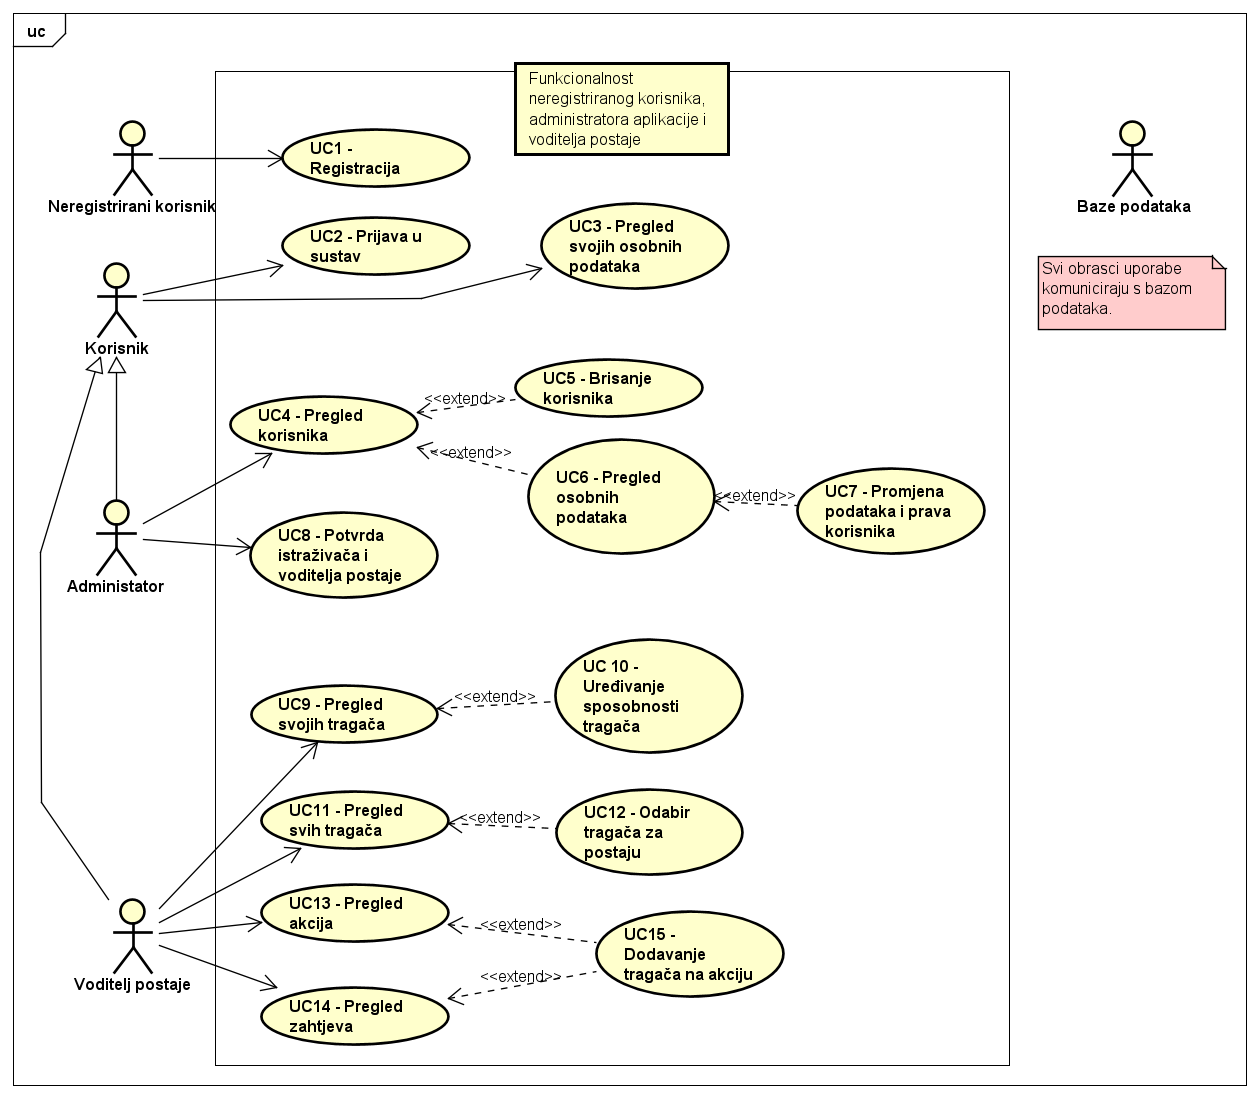
\includegraphics[scale=0.5]{slike/dijagram admin.png} %veličina slike u odnosu na originalnu datoteku i pozicija slike
						\centering
						\caption{Funkcionalnost neregistriranog korisnika, generaliziranog korisnika, administratora aplikacije i voditelja postaje}
						\label{fig:Funkcionalnost neregistriranog korisnika, administratora aplikacije i voditelja postaje}
					\end{figure}
					
					\begin{figure}[H]
						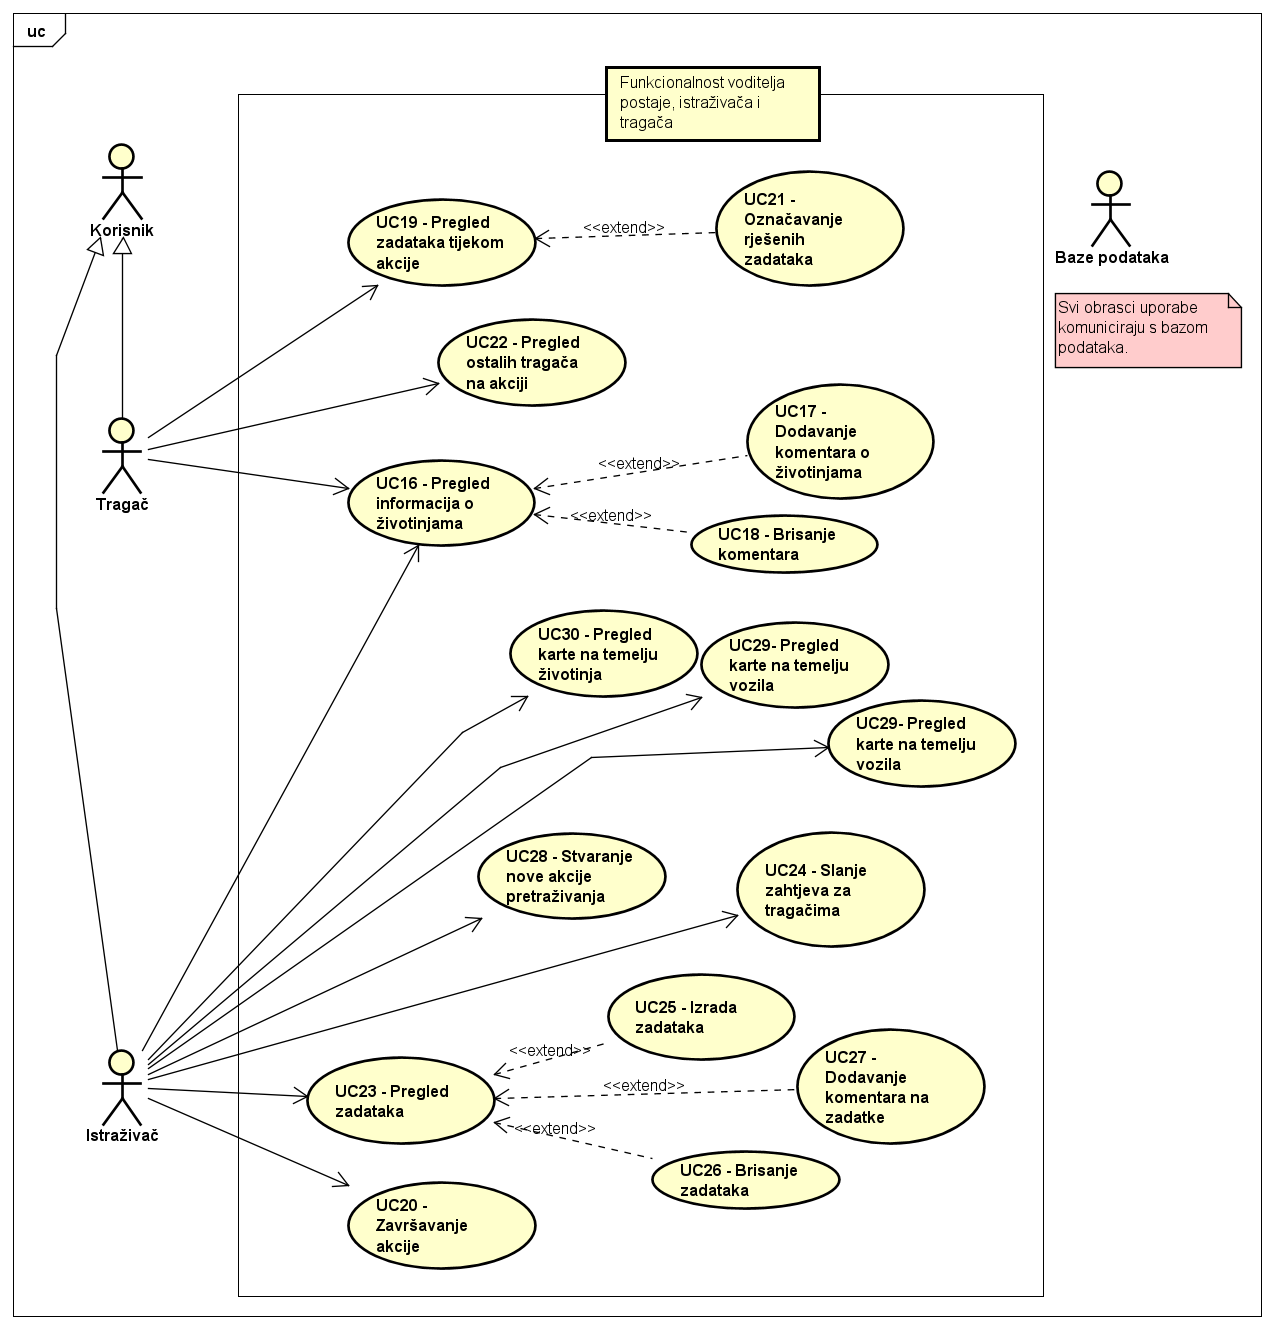
\includegraphics[scale=0.5]{slike/dijagram ekipa.png} %veličina slike u odnosu na originalnu datoteku i pozicija slike
						\centering
						\caption{Funkcionalnost tragača i istraživača}
						\label{fig:Funkcionalnost tragača i istraživača}
					\end{figure}
				
					\eject		
				
			\subsection{Sekvencijski dijagrami}
				
				\noindent 
				\textbf{Obrazac uporabe UC1 - Registracija}\\

				\noindent 
				Neregistrirani korisnik šalje zahtjev za registracijom. Aplikacija dohvaća popis registriranih korisnika
        				iz baze podataka.
        				Ako korisnik nije na popisu aplikacija mu šalje potvrdu na mail koju korisnik mora potvrditi.
        				U slučaju da se korisnik registrira da bi bio voditelj postaje ili istraživač aplikacija šalje administratoru
        				zahtjev za potvrdom te administrator mora potvrditi registraciju.
        				Zatim aplikacija zapisuje podatke u bazu podataka te dobiva potvrdu o uspjehu registracije od baze podataka
        				te aplikacija korisniku prikazuje poruku o uspješnoj registraciji.
        				Ako korisnik postoji u bazi podataka aplikacija, korisnik se obavještava da korisnik već postoji u bazi podataka.

				
				
				\begin{figure}[H]
					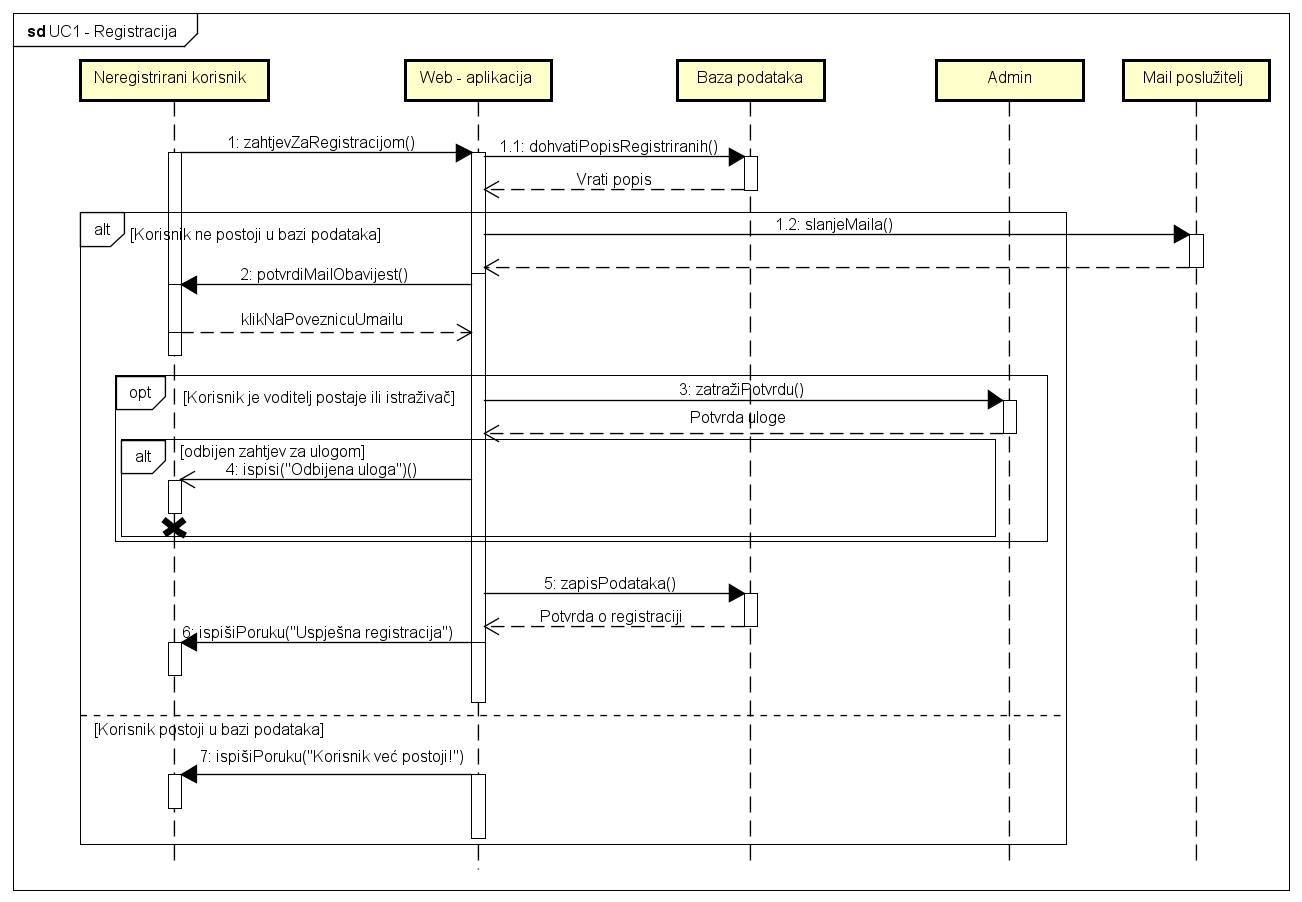
\includegraphics[scale=0.5]{slike/UC1 - Registracija.png} %veličina slike u odnosu na originalnu datoteku i pozicija slike
					\centering
					\caption{Sekvencijski dijagram za UC1}
					\label{fig:UC1 - Registracija}
				\end{figure}

				\eject

				\noindent
				\textbf{Obrazac uporabe UC19 - Dodavanje tragača na akciju}\\

				\noindent
				Voditelj postaje šalje aplikaciji upit za novim akcijama.
        			Aplikacija dohvaća popis aktivnih akcija iz baze podataka te ih prikazuje voditelju postaje.
        			Voditelj postaje zatim prolazi kroz sve aktivne akcije.
        			Aplikacija iz baze podataka dohvaća sve slobodne tragače koji zadovoljavaju zahtjeve istraživača.
        			U slučaju da ne postoje takvi tragači voditelju se postaje ispisuje poruka da nema dostupnih tragača.
        			U slučaju da popis nije prazan voditelju postaje prikazuje se popis tragača.
        			Voditelj postaje potom šalje odabrane tragače aplikaciji koja zatim dodaje akciju tragaču u bazi podataka te
        			vraća voditelju postaje obavijest da je zahtjev poslan tragaču.

				

				\begin{figure}[H]
					\includegraphics[scale=0.5]{slike/UC19 - Dodavanje tragača na akciju.png} %veličina slike u odnosu na originalnu datoteku i pozicija slike
					\centering
					\caption{Sekvencijski dijagram za UC19}
					\label{fig:UC19 - Dodavanje tragača na akciju}
				\end{figure}
	
				\eject

				\noindent
				\textbf{Obrazac uporabe UC24 - Završavanje akcije}\\

				\noindent
				Tragač šalje aplikaciji zahtjev za krajem akcije.
        				Aplikacija dohvaća popis zadataka iz baze podataka i prikazuje popis tragaču.
        				Ako popis nije prazan tragaču se ispisuje poruka da nisu svi zadatci riješeni.
				        Ako je popis prazan aplikacija šalje bazi podataka zahtjev za krajem akcije
        				te potom obavještava tragača da je akcija završena.

				

				\begin{figure}[H]
					\includegraphics[scale=0.6]{slike/UC24 - Završavanje akcije.png} %veličina slike u odnosu na originalnu datoteku i pozicija slike
					\centering
					\caption{Sekvencijski dijagram za UC24}
					\label{fig:UC24 - Završavanje akcije}
				\end{figure}

				\eject

				\noindent
				\textbf{Obrazac uporabe UC37 - Stvaranje nove akcije pretraživanja}\\

				\noindent
				Istraživač aplikaciji šalje zahtjev za novom akcijom.
				        Aplikacija provjerava ima li istraživač već aktivne akcije.
        				U slučaju da istraživač već ima aktivnu akciju aplikacija obavještava istraživača da već postoji aktivna akcija.
        				Ako istraživač nema aktivnu akciju aplikacija bazi podataka šalje zahtjev za dodavanjem nove akcije te se
        				istraživač obavještava da je akcija uspješno stvorena.

				

				\begin{figure}[H]
					\includegraphics[scale=0.5]{slike/UC37 - Stvaranje nove akcije pretraživanja.png} %veličina slike u odnosu na originalnu datoteku i pozicija slike
					\centering
					\caption{Sekvencijski dijagram za UC37}
					\label{fig:UC37 - Stvaranje nove akcije pretraživanja}
				\end{figure}

				\eject
	
		\section{Ostali zahtjevi}

		\begin{packed_item}
			\item Sustav treba podržavati istovremeni rad više korisnika u stvarnom vremenu
			\item Korisničko sučelje i sustav moraju podržavati hrvatsku abecedu 
			\item Pristup bazi podataka trebao bi biti učinkovit, s vremenom izvršavanja unutar nekoliko sekundi
			\item Za izradu sustava kao web aplikacije, koriste se objektno-orijentirani jezici
			\item Pogrešna uporaba korisničkog sučelja ne bi smjela imati negativan utjecaj na funkcionalnost i rad sustava
			\item Sustav treba biti jednostavan za korištenje
			\item Pri nadogradnji sustava, ne smiju se narušavati postojeće funkcionalnosti
			\item Veza s bazom podataka mora biti zaštićena, brza i otporna na vanjske greške
			\item Pristup sustavu treba biti moguć iz javne mreže, uz korištenje HTTPS-a radi sigurne komunikacije
		\end{packed_item}
	